\chapter{Results}
\label{chap:results}

In this chapter we present results from the evaluation phase.

\section{Data separation}
For evaluation and testing purposes, access was given to a CIMS instance with a database containing about 3 years worth of data, where the largest table (job event) contains about 480 million rows. Using the developed software components for transforming and migrating data, all relevant data from the CIMS instance was moved to the databases of the archive prototypes. Some measurements were done during the migration process, specifically how much time the process took. This was done mainly to get ball park figures to answer if the expected time is likely to be hours, days or weeks.



\section{Query support}

The set of important queries defined in section~\ref{sec:usecases} has been implemented for the archive prototypes using mongodb and elasticsearch. In this section the results of this implementation are presented.

\hiddensubsection{Get build}

\hiddensubsection{Get build information}

\hiddensubsection{Get build for root test suite}

\hiddensubsection{Get trouble reports for build}

\hiddensubsection{Get trouble report fixes for build}

\hiddensubsection{Get trouble reports for product and revision}

\hiddensubsection{Get test suite children}

\hiddensubsection{Get test case in build}

\hiddensubsection{Get test suite in build}

\hiddensubsection{Get root test suite for test case/test suite}

\hiddensubsection{Get test case by name}

\hiddensubsection{Get test suite for test case}

\hiddensubsection{Get test case history}

\hiddensubsection{Get test tree}

\hiddensubsection{Get all build data}

%\begin{table}[h]
%\begin{tabular}{|l|l|l|}
%\hline
%\textbf{High level query}                & \textbf{Supported} & \textbf{Comment}           \\ \hline
%Get build                                    & Y                                                                                        &                            \\ \hline
%Get build information                        & Y                                                                                        &                            \\ \hline
%Get build for root test suite                & Y                                                                                        &                            \\ \hline
%Get trouble reports for build                & Y                                                                                        &                            \\ \hline
%Get trouble report fixes for build           & Y                                                                                        &                            \\ \hline
%Get trouble reports for product and revision & Y                                                                                        &                            \\ \hline
%Get test suite children                      & Y                                                                                        &                            \\ \hline
%Get test case in build                       & Y                                                                                        &                            \\ \hline
%Get test suite in build                      & Y                                                                                        &                            \\ \hline
%Get root test suite for test case/test suite & Y                                                                                        &                            \\ \hline
%Get test case by name                        & Y                                                                                        & Used for test case history \\ \hline
%Get test suite for test case                 & Y                                                                                        &                            \\ \hline
%Get test case history                        & P                                                                                        & Tags not supported         \\ \hline
%Get test tree                                & P                                                                                        & Runs slow for large trees  \\ \hline
%\end{tabular}
%\caption{Possible values in the supported column are yes/no/partially.}
%\label{tab:archivequeries}
%\end{table}

%\section{Schema evolution}
%Not yet addressed

\section{Scalability}
\subsection{Disk usage}
Disk usage after migration of live databases of different sizes are presented in figure~\ref{fig:disc}. 
The first migration that was performed was that of the previously mentioned CIMS instance with 480 million rows in the job event table. Size is presented in the figure~\ref{fig:disc}. This is the largest database with real data that could be used for evaluation purposes. In order to perform larger migrations, dummy job event data was generated in range of 2 to 3 billion documents/rows and inserted into the archive databases.
\begin{figure}[h!]
\centering
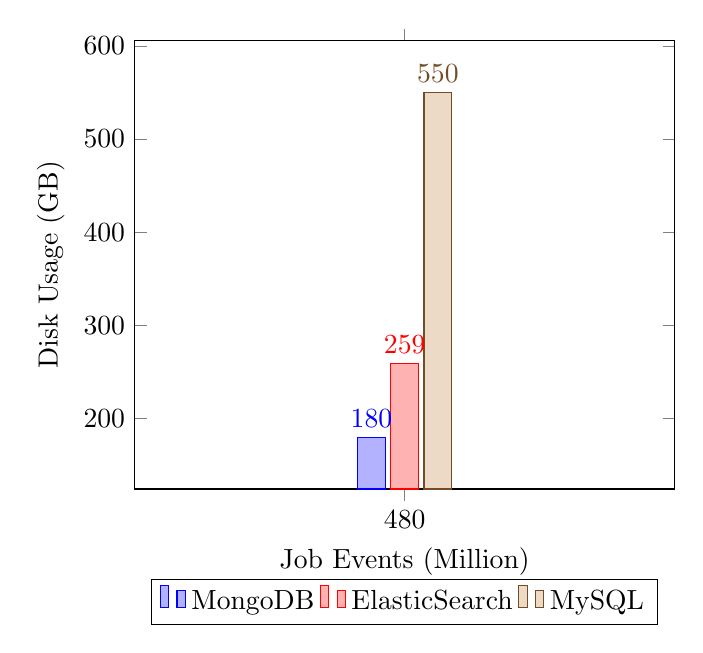
\begin{tikzpicture}
\begin{axis}[
    ybar,
    enlargelimits=0.15,
    legend style={at={(0.5,-0.2)},
      anchor=north,legend columns=-1, },
    xlabel={Job Events (Million)},
    ylabel={Disk Usage (GB)},
    symbolic x coords={480},
    xtick=data,
    nodes near coords,
    nodes near coords align={vertical},
    ]
\addplot coordinates {(480,180)};
\addplot coordinates {(480,259)};
\addplot coordinates {(480,550)};
\legend{MongoDB,ElasticSearch,MySQL}
\end{axis}
\end{tikzpicture}
\caption{Disk usage after migrating data from CIMS instance with real data.}
\label{fig:disc}
\end{figure}

\begin{figure}[h!]
\centering
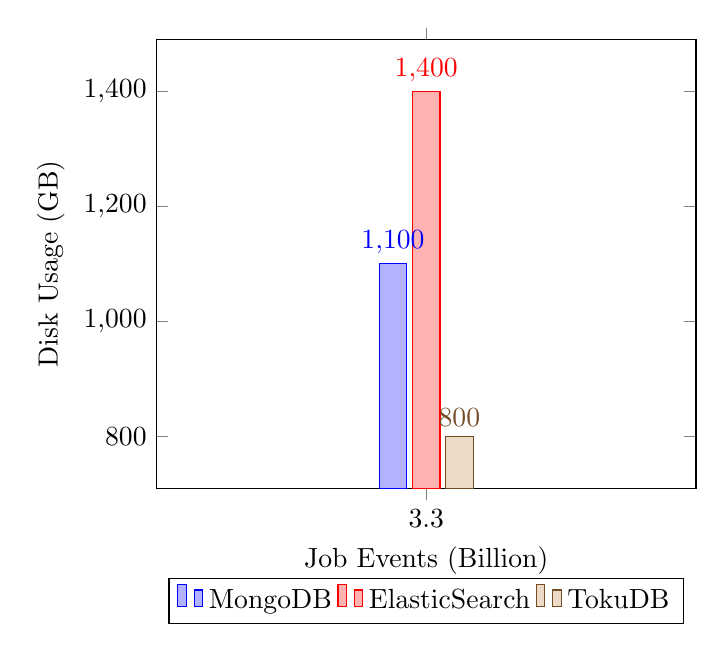
\begin{tikzpicture}
\begin{axis}[
    ybar,
    enlargelimits=0.15,
    legend style={at={(0.5,-0.2)},
      anchor=north,legend columns=-1, },
    xlabel={Job Events (Billion)},
    ylabel={Disk Usage (GB)},
    symbolic x coords={3.3},
    xtick=data,
    nodes near coords,
    nodes near coords align={vertical},
    ]
\addplot coordinates {(3.3, 1100)};
\addplot coordinates {(3.3, 1400)};
\addplot coordinates {(3.3, 800)};
\legend{MongoDB,ElasticSearch,TokuDB}
\end{axis}
\end{tikzpicture}
\caption{Disk usage after having a combination of real data and generated data.}
\label{fig:discbig}
\end{figure}

\subsection{Memory utilization}
\hiddensubsubsection{Insertion}


\hiddensubsubsection{Query}
Working set estimations are presented in figure~\ref{fig:ws}. Initial estimations of the working set for MongoDB have been done with manual testing. As long as custom indexes defined on the job event collection fit in RAM, the database is stable and can respond to queries where indexes can be utilized. The working set estimation is the summed size of the custom indexes.

\begin{figure}[h!]
\centering
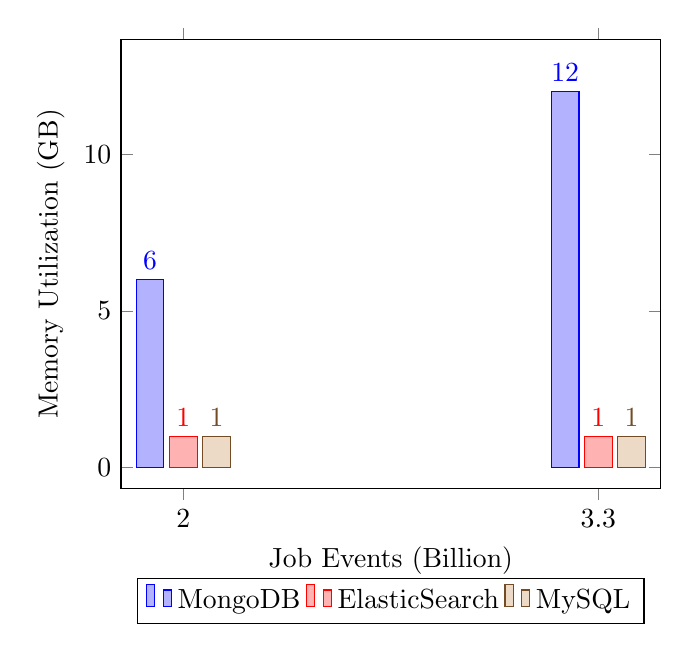
\begin{tikzpicture}
\begin{axis}[
    ybar,
    enlargelimits=0.15,
    legend style={at={(0.5,-0.2)},
      anchor=north,legend columns=-1, },
    xlabel={Job Events (Billion)},
    ylabel={Memory Utilization (GB)},
    symbolic x coords={2,3.3},
    xtick=data,
    nodes near coords,
    nodes near coords align={vertical},
    ]
\addplot coordinates {(2,6) (3.3,12)};
\addplot coordinates {(2,1) (3.3,1)};
\addplot coordinates {(2,1) (3.3,1)};
\legend{MongoDB,ElasticSearch,MySQL}
\end{axis}
\end{tikzpicture}
\caption{Working set estimation}
\label{fig:ws}
\end{figure}
\subsection{Insertion time}
Migrations were first performed in an environment where many developers share the same resources. The process then took between 4 and 5 days to complete.

After switching to a dedicated server with 256GB of RAM and 48 CPU's, the migration process took less than a day for elasticsearch.

\subsection{Horizontal Scalability}
Not yet addressed
Här borde vi kunna skriva tekniska saker, men från de tekniska saker dra slutsater i Discussion som svarar på om dessa tekniker ger något business value?
\hiddensubsubsection{MongoDB}
\hiddensubsubsection{Elasticsearch}
"Lessons learned while scaling with Elasticsearch, future work can be to test with more nodes".\\
Compared to MongoDB, horizontal scaling with Elasticsearch demands more configuration upfront in order to get a suitable cluster. 
In MongoDB, where the process of adding new nodes to a cluster is not limited on how the initial node is configured, the maximum number of nodes in an Elasticsearch cluster must be known on beforehand. This restriction depends on how Elasticsearch is scaling in an horizontal manner. The partitioning of data when adding new nodes to a cluster is dependent on how many shards the initial node holds, as an new node is added to the cluster it overtakes shards from the already existing nodes.

\hiddensubsubsection{TokuDB}
\section{Organizational suitability}
This section describes the organizational suitability of the different artifacts.
\hiddensubsection{MongoDB}
\hiddensubsection{Elasticsearch}
\hiddensubsection{TokuDB}